%----------------------------------------------------------------------
\section{Introduction}\label{sec:intro}
%----------------------------------------------------------------------

% \Ethan{TODO fix the story.}
% \begin{enumerate}
%     \item Why external solver?
%     \begin{itemize}
%         \item For certain codes (e.g. bicycle bivariate code),
%         the best known distance verification algorithm runs in exptime.
%         Lean by itself is too ``slow'' to deal with these NP-hard things.
%         \item Another project \cite{feng-9-qubits} tried it the hard way
% anyways.
%         Didn't scale past 9 qubits, before enumerating and analyzing each
% possible error ($9\times\abs{\set{X, Y, Z}}=27$) by hand became too much.
%     \end{itemize}
%     \item The na\"ive Lean formalization of code distance does \emph{not}
% scale either.
%     Instantiating the Boolean formula (i.e. before even invoking a solver)
% became intractable due to the sheer numbers of variables and clauses.
%     In order to reach 72 qubits \Ethan{and probably beyond -- need to run more
% experiments}, we add an additional intermediate QEC representation, and prove
% that our representation is consistent with the \lstinline{Matrix}-based golden
% reference.
%     \item Na\"ively translating the distance formalism into a Boolean formula
% is no good either.
%     (Anecdotal evidence: 72 qubit fine outside Lean.
%     90 might need cluster. 144 completely intractable.)
%     After several iterations, we arrived at a Boolean formula that scales to
% 72 qubits with Lean's proof construction overhead,
%     as well as 144 qubits outside of Lean.
% \end{enumerate}
%
% \Ethan{above are the potentially interesting facts}
%
% Quantum computing is a model of computing built on quantum mechanical
% principles, using continuous-valued ``qubits'' instead of discrete bits and
% allowing for entanglements between different qubits. At scale, quantum
% computers will outperform classical computers in a number of domains by
% significant asymptotic advantages, with great applications in cryptography,
% physics, chemistry, and optimization \cite{shor1999polynomial,
% berry2007efficient, mcardle2020quantum, harrow2009quantum}. Quantum computers
% are difficult to build because qubits are much harder to build and control
% than classical bits, and are vulnerable to greater amounts of noise that is at
% the same time more complicated than traditional bit error models. This
% complicates programs run on quantum computers because they must pass through a
% complicated layer of Quantum Error Correction (QEC). As we move beyond the
% NISQ era \cite{Preskill_2018}, there are an increasing number of real-time
% experimental demonstrations of Quantum Error Correction
% \cite{google2023suppressing, postler2024demonstration, google2025quantum}.
% Because of the complex nature and high importance of our fault-tolerant
% quantum programs it is reasonable that we should seek to obtain confidence in
% their function through verification.
%
% For classical programs extensive testing is used to ensure correctness.
% However, quantum states in general are exponentially large, and protocols for
% checking their properties called Quantum State Tomography require
% exponentially many copies of the state in the general case and thus are
% prohibitively expensive. Moreover, due to the laws of quantum physics,
% mid-circuit measurements would collapse the quantum state, making breakpoints
% or runtime assertions impossible.
%
% From these limitations, an effective way to gain confidence in quantum
% programs is to \emph{formally verify} their semantics. Formal verification is
% a method of defining strict, mathematically sound requirements for a system,
% and using a trusted tool to show that the system satisfies those requirements.
% In classical computing, formal verification has found wide adoption in
% industrial applications with critically important code, and similar techniques
% in mathematics have allowed for large scale proof checking and buttressed
% recent advances in AI theorem proving \cite{demoura2021, mathlib2020,
% achim2025aristotle}.
%
%
% In quantum computing, there are a number of recent works applying verification
% to program correctness, error correction, and quantum information theory
% \cite{amy2018towards, huang2025efficient, meiburg2025formalization}. While
% these works provide useful results, they are separate efforts individual steps
% of quantum computing and are not connected.
% Indivdual verification and formalization of disconnected parts of a model are
% significantly less useful than an \textbf{end-to-end} formalization
% encompassing those parts. For any model consisting of individually verified
% portions, there is always a chance of correctness being ``lost in
% translation'' between those verified parts. Additionally, having the model
% entirely within one formalization allows for cross-layer reasoning at times
% when higher-level formalizations aren't powerful enough to solve problems.
%
% Recently, Peng et al. \cite{peng2022formallycertifiedendtoendimplementation}
% have been able to verify end-to-end properties of quantum algorithms like
% Shor's Algorithm, but the full picture for quantum computing is more
% complicated.
%
% Creating a more trustworthy form of formal verification for Quantum Computing
% faces the following challenges, which are addressed in this work.
%
% \begin{enumerate}
%     \item \textbf{Noise Model:}
%
%     Due to the presence of noise, it does not suffice to verify that a quantum
% circuit performs its desired operation on an idealized circuit model. Instead,
% the performance of the circuit under the presence of a certain degree of noise
% must be verified, namely through verifying the efficacy of QEC.
%
%     \item \textbf{Translation between circuits through QECC:}
%
%     Error corrected circuits do not look the same on physical hardware as they
% do before error correction. The process of making a circuit fault-tolerant
% replaces every operation with logically equivalent "gadgets" that are designed
% to resist noise and correctly implement the given operation.
%
%     \item \textbf{End-to-end Connectivity:}
%
%     As discussed earlier, full confidence cannot be obtained through
% verification that is not end-to-end. However, most theorems are not proven
% with the end-to-end picture in mind. Instead, they are proven with respect to
% some formalism that abstracts away certain elements. Thus, a nontrivial amount
% of "glue" work is required to make separate theories fit together.
%
%     \item \textbf{Computational Hardness:}
%
%     Formalization of code properties in Quantum Error Correction are not only
% mathematically hard to understand by humans, but also \emph{computationally}
% hard. For example, determining the code distance of a stabilizer code
% displaying little symmetry is exponentially hard, as determining the distance
% of \textit{classical} error-correcting codes in general is hard
% \cite{vardy2002intractability}. Normally, code parameters would be fed into a
% computer program such as a linear integer programming (IP) solver or
% specialized QECC software, and someone making use of the values would copy
% them over to their theory.
% \end{enumerate}
%
% Using the modular properties of Lean as a programming language for
% representing complex mathematical ideas, we envision a program for formally
% verifying quantum circuits that combines formal verification of the error
% correction protocols with formal verification of the behavior of the logical
% circuit to represent the entire behavior of the quantum computer.
%
% In this work, we introduce \textbf{Lean-QEC}, a library for end-to-end
% verification of Quantum Error-Correcting Codes using Lean. Overall we make the
% following contributions.
% \begin{enumerate}[leftmargin=1.5em]
%   \item \textbf{A modular end-to-end framework for formally verifing the
% theory of Quantum Error Correction}, including Pauli Group theory, stabilizer
% codes, the binary symplectic representation, and how these theories relate to
% code properties like distance.
%
%   \item \textbf{A SAT-assisted distance verification pipeline} that verifiably
% translates quantum-theoretic code distance statements through the binary
% symplectic representation into Boolean+Integer satisfiability problems, and
% uses Lean's SAT integration to call an external solver and reconstruct its
% proof in Lean.
%
%
%   \item \textbf{End-to-end verification of industry-level error correction
% codes}. We formalize and verify specific code families like CSS Codes,
% Bivariate Bicycle Codes, demonstrating application of formalization and ease
% of obtaining concrete code distance results. This allows us to obtain higher
% confidence in QECC results and is an important step towards the practical
% end-to-end verification of quantum circuits.
%
% \end{enumerate}
%
%
% To further motivate an end-to-end formalization, one may imagine a
% formalization of stabilizer codes using the stabilizer binary symplectic
% representation as a primitive. The notion of distance may be understood
% according to its stabilizer-theoretic definition, and many in-principle
% similar results to what has been obtained in this paper could be verified.
% However, the truth of the verification would no longer entirely rest on the
% Lean kernel, as ours does. Instead, it would depend on the informally
% understood mathematical equivalences between the binary symplectic
% representation and the quantum-theoretic definition, in which the stabilizer
% code is actually a simultaneous $+1$ eigenspace of a set of Pauli matrices.
%
% We stress the unification of these formalisms performed in our library.
% Importantly, our formalization is able to make use of the binary symplectic
% representation through \textit{formally proving} its correspondence to the
% stabilizers themselves in Lean. Then, we may to come to the same conclusions
% drawn from the formalism, but through our correspondence theorems may pass
% backwards to relate the statements to their expanded mathematical meaning.
% This end-to-end methodology allows one to reap the same benefits as a
% disconnected formalization, so long as the disconnected formalizations may
% actually be performed within the given end-to-end environment.
%
% \Ethan{I think we need to link our GitHub somewhere?
% Give the usual spiel of having open source code and whatnot?}
%

Quantum computing promises asymptotic speedups on classically intractable
problems in cryptography, simulation, optimization, and
chemistry~\cite{shor1999polynomial, berry2007efficient, mcardle2020quantum,
harrow2009quantum}. Realizing those speedups on real hardware, however, is
constrained by noise: every physical qubit decoheres and every physical gate is
imperfect~\cite{Preskill_2018}, so the only known route to scalable computation
passes through a thick layer of \emph{quantum error correction} (QEC). Recent
experimental demonstrations of QEC on superconducting and trapped-ion
platforms~\cite{google2023suppressing, postler2024demonstration,
google2025quantum} have made this layer a load-bearing component of the quantum
stack rather than a theoretical curiosity, and have accordingly raised the bar
for the trust placed on it.

The classical engineering response to such load-bearing code is testing, but
testing is essentially unavailable for quantum programs. Output distributions
are exponentially expensive to sample, intermediate measurements collapse the
very state under inspection, and the noise that motivates correction also
corrupts any would-be observation. The remaining option is to \emph{formally
verify} the QEC layer~\cite{demoura2021, mathlib2020}: state its guarantees as
theorems and discharge them in a proof assistant whose kernel can be
independently trusted.

\paragraph{Why the distance number is hard to trust.} The most informative
single parameter of a stabilizer code is its \emph{distance} $d$: the minimum
Pauli weight of an undetectable error. A code with distance $d$ corrects
$\lfloor(d-1)/2\rfloor$ errors, so distance is the value most often quoted when
codes are compared and the value on which fault-tolerance thresholds depend. Yet
certifying a distance lower bound is computationally hard: even for classical
linear codes the problem is NP-complete~\cite{vardy2002intractability}, and for
stabilizer codes lacking strong symmetry the situation inherits the same
intractability \cite{Kapshikar_2023}. The values quoted in the literature therefore come from one of
two unsatisfying places:
\begin{itemize}[leftmargin=1.5em]
    \item \textbf{Hand proofs inside a proof assistant.} Existing developments
    such as the 9-qubit Shor-code verification~\cite{feng-9-qubits} enumerate
    every Pauli error explicitly. The bookkeeping --- $3n$ single-qubit error
    patterns plus all of their combinations --- has so far prevented this style
    from scaling past nine qubits, well short of any code used in current
    experiments.
    \item \textbf{Unverified symbolic computation.} ILP solvers, custom search
    routines, or computer-algebra scripts can in principle handle larger codes~\cite{webster2026distancefindingalgorithmsquantumcodes}, 
    but their outputs sit entirely outside the proof kernel. A distance value
    pasted from such a tool is the moral equivalent of a numerical constant
    trusted on faith.
\end{itemize}
Neither option is end-to-end: the first does not scale, and the second leaves a
trust gap at exactly the point the code is meant to provide a guarantee.

\paragraph{Why end-to-end matters.} A pragmatic shortcut is to declare a
stabilizer code by its binary symplectic representation and treat distance as a
property of that matrix. This makes the math tractable, but it shifts the trust
to an informal equivalence between two definitions --- the matrix view and the
original quantum-theoretic view in which a stabilizer code is the simultaneous
$+1$ eigenspace of a set of Pauli matrices. A genuinely trustworthy artifact
must close that loop inside the proof kernel: distance bounds proved over the
matrix view must transport, by a machine-checked theorem, to the eigenspace
view.

\paragraph{Our approach.} We present \textsc{Lean-QEC}, a Lean~4 library that
builds the stabilizer-code stack end-to-end and discharges distance certificates
against industrial-scale codes by combining the proof assistant with an external
SAT solver. The library covers the linear algebra of qubit states, the Pauli
group with phases, stabilizer codes, the binary symplectic representation,
classical coding theory, CSS codes, and the Bivariate Bicycle (BB) family. Each
abstraction layer is connected to the next by a machine-checked correspondence
theorem, so a distance bound established on a binary symplectic matrix is also a
theorem about the corresponding quantum code.

For the computationally hard step, \textsc{Lean-QEC} reduces ``distance $\geq
d$'' to the unsatisfiability of a Boolean formula via a Lean-verified
translation, hands the formula to CaDiCaL through Lean's \lstinline{bv_decide}
tactic, and reconstructs the resulting LRAT certificate as a Lean proof term.
The trusted base remains Lean's kernel plus the LRAT checker; the SAT solver
itself is not trusted.

Making this pipeline scale required two non-obvious design moves, both of which
we present as contributions in their own right:
\begin{enumerate}[leftmargin=1.5em]
    \item Instantiating the Boolean formula directly through Mathlib's
    \lstinline{Matrix} type exhausts memory well before reaching the
    $[[90,8,10]]$ BB code. We introduce a \lstinline{BitVec}-flattened
    intermediate representation, prove it consistent with the
    \lstinline{Matrix}-based reference, and use it to carry the encoding past the 90-qubit mark.
    \item Even with an efficient encoding, a one-Boolean-per-qubit error
    variable produces a formula whose solver runs become intractable beyond
    about 90 qubits. We instead let the variables encode the \emph{locations} of
    the (at most $d-1$) nonzero error entries, shrinking the variable count from
    $n$ to $k\lceil\log_2 n\rceil$. For the $[[144,12,12]]$ BB code this is $88$
    variables versus $144$ --- a difference that makes 144 qubits tractable
    outside the kernel in minutes.
\end{enumerate}

\paragraph{Contributions.} Our contributions are as follows.
\begin{enumerate}[leftmargin=1.5em]
  \item \textbf{An end-to-end Lean~4 formalization of stabilizer-code theory.}
  We give a machine-checked development that connects qubit states, the Pauli
  group with phases, stabilizer codes, the binary symplectic representation, and
  classical coding theory, with explicit correspondence theorems between
  adjacent layers (\Cref{sec:QECBackground}).

  \item \textbf{A verified reduction from code distance to Boolean
  satisfiability.} We formalize a translation from the stabilizer-theoretic
  distance condition to an UNSAT query, prove the reduction sound in Lean, and
  integrate it with Lean's \lstinline{bv_decide} tactic so the SAT certificate
  is reconstructed in the kernel (\Cref{sec:smt}).

  \item \textbf{Two scalability techniques.} A \lstinline{BitVec}-based
  intermediate representation, verified consistent with the \lstinline{Matrix}
  encoding, lets the formula instantiation reach industrial code sizes; a
  location-indexed error encoding cuts the SAT variable count from $n$ to
  $k\lceil\log_2 n\rceil$ (\Cref{sec:translation}).

  \item \textbf{Lean-checked distance certificates for practical codes.} We
  instantiate the pipeline on industrially viable codes like the $[[90,8,10]]$ Bivariate Bicycle code of \cite{bravyi2024} and the $[[70, 6, 9]]$ BB code of \cite{tripier2026faulttolerantquantumcomputingtrapped}, and report the
  resource envelope outside Lean for the Gross Code of size $[[144,12,12]]$. Each case study is between
  $100$ and $200$ lines of Lean script and follows a uniform template
  (\Cref{sec:casestudies}), which may be automatically generated by a Python script given the code description.
\end{enumerate}

\paragraph{Comparison.} \Cref{tab:comparison} summarizes how \textsc{Lean-QEC}
sits relative to the two existing options. Hand-written ITP proofs of distance
close the trust loop but stall well below twenty qubits; unverified solver
pipelines reach industrial codes but never enter the kernel. \textsc{Lean-QEC}
closes the loop \emph{and} reaches industrial codes by paying for the solver
call with a verified reduction and a reconstructed certificate.

\begin{figure}[t]
    \centering
    \vspace{-1.25cm}
    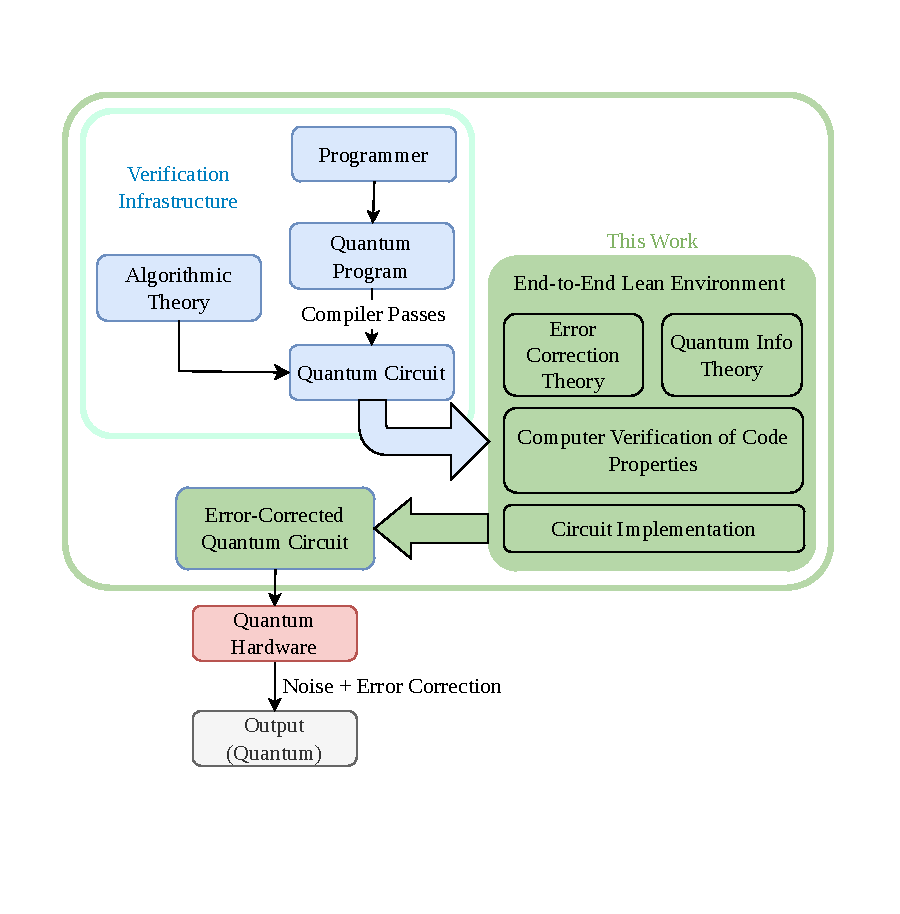
\includegraphics[width=0.9\linewidth]{Figures/qflow.drawio.pdf}
    \vspace{-2cm}
    \caption{Verification workflow for fault-tolerant quantum programs.
    \textsc{Lean-QEC} occupies the QEC layer of this pipeline.}
    \label{fig:qflow}
\end{figure}

\begin{table}[ht]
\small
\centering
\caption{Comparison of verification approaches for QEC
distance.}\label{tab:comparison}
\begin{tabular}{@{}lccc@{}}
\toprule
\textbf{Approach} & \textbf{Theory verified?} & \textbf{Scales to large codes?} & \textbf{End-to-end checked?} \\
\midrule
Hand-written ITP proofs         & Yes & No ($n > 20$ prohibitive) & Yes \\
Unverified symbolic computation & No  & Yes                       & No  \\
\textsc{Lean-QEC} (this work)   & Yes & Yes (${\sim}2^{40}$ cases) & Yes \\
\bottomrule
\end{tabular}
\end{table}


The rest of the paper develops \textsc{Lean-QEC} in the order a quantum
researcher would encounter the abstractions: \Cref{sec:fv} introduces just
enough Lean to follow the formalization; \Cref{sec:QECBackground} builds the QEC
stack with explicit attention to the type-theoretic gaps that arise when
formalizing standard quantum-information arguments; \Cref{sec:smt} presents the
SAT-assisted distance pipeline; \Cref{sec:casestudies} reports the case studies;
and \Cref{sec:Conclusion and Discussion} discusses related work and limitations.
